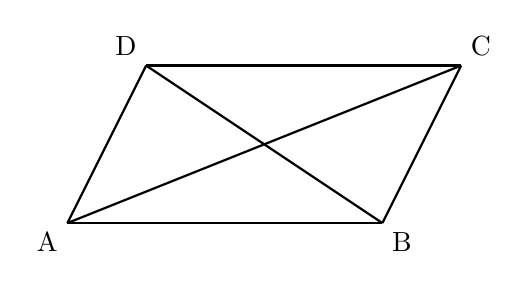
\begin{tikzpicture}

    % Define the coordinates for parallelogram ABCD
    \coordinate (A) at (0, 0);       % Bottom left vertex
    \coordinate (B) at (4, 0);       % Bottom right vertex
    \coordinate (C) at (5, 2);       % Top right vertex
    \coordinate (D) at (1, 2);       % Top left vertex
    
    % Draw the parallelogram sides
    \draw[thick] (A) -- (B);         % Side AB
    \draw[thick] (B) -- (C);         % Side BC
    \draw[thick] (C) -- (D);         % Side CD
    \draw[thick] (D) -- (A);         % Side DA
    
    % Draw the diagonals
    \draw[thick] (A) -- (C);         % Diagonal AC
    \draw[thick] (D) -- (B);         % Diagonal DB
    
    % Label point A
    \node[below left] at (A) {A};
    
    % Label point B
    \node[below right] at (B) {B};
    
    % Label point C
    \node[above right] at (C) {C};
    
    % Label point D
    \node[above left] at (D) {D};
    
    \end{tikzpicture}